\chapter{Learning of Boltzmann machines}

\section{Unsupervised learning}
So far it was assumed that the couplings in analysed structures (along with bias terms) were known a priori. However, in general when we analyse some phenomena we don't know this values and we are interested in learning an unknown distribution $Q$ based on some observed data $\mathcal{D}$. The theoretical results suggests that the RBM structure is a natural candidate for approximating underlying distribution from which the data were generated. Thus, the unsupervised learning in this case consists of learning the parameters $\theta$ of the approximate distribution $P$. Therefore, our general goal is to maximize the probability of $\mathcal{D}$ under the MRF distribution i.e. we are looking for the vector of parameters $\mathbf{\theta}$ that maximize the likelihood given the training data:
\begin{align}
\begin{split}
\max_{\mathbf{\theta}} \ln \mathcal{L}(\mathbf{\theta}| \mathcal{D}) = \max_{\mathbf{\theta}}  \ln \prod_{i=1}^N p(\mathbf{v}_i |\mathbf{\theta}) = \max_{\mathbf{\theta}} \sum_{i=1}^N \ln p(\mathbf{v}_i |\mathbf{\theta} )
\end{split}
\end{align}
where $N$ is the size of $\mathcal{D}$. 

The experiments on toy models suggest that the initial unsatisfactory results with naive mean field approaches \cite{tieleman2008training} might be greatly improved if we include additional terms responsible for connections between the spins.

\section{Training of Boltzmann Machines}
With large graphical models, it is not possible to find an analytical solution to the maximum likelihood estimation of parameters and we need to resort to some approximation methods. That is also the case of the RBM and learning the parameters of this structure relies on the gradient ascent of the log-likelihood. At time $t$ during training, the update of the vector containing all parameters of the RBM $\mathbf{\theta}$ has the form:
\begin{align}
\begin{split}
\mathbf{\theta}^{t} = \mathbf{\theta}^{t-1} + \eta  \frac{\partial}{\partial \mathbf{\theta}^{t-1}}  \ln \mathcal{L}(\mathbf{\theta}| \mathcal{D}). 
\end{split}
\end{align}
This relies on the fact that the gradient w.r.t. parameters $\mathbf{\theta}$ informs us how fast function increases in the current point $\mathbf{\theta}^{t-1}$. 
By taking appropriately small learning rate, these iterative updates converge to stationary points. With large data set it is common to use a stochastic gradient ascent method \cite{robbins1951stochastic} where we sample a minibatch of datapoints and take a noisy gradient estimate which results in the update rule:
\begin{align}
\begin{split}
\mathbf{\theta}^{t+1} = \mathbf{\theta}^{t} + \eta \frac{1}{M} \frac{\partial}{\partial \mathbf{\theta}^t}  \sum_{m =1}^{M} \ln \mathcal{L}(\mathbf{\theta}| \mathbf{x}^{(m)}),
\end{split}
\label{eq:sgd}
\end{align}
where $M$ is the size of the minibatch. It can be shown that updates via \ref{eq:sgd} guarantee to converge to a local optimum under weak conditions \cite{bottou1998online}.

For a given data point $\mathbf{v}$ the log-likelihood can be seen as the difference between two energies:
\begin{align}
\begin{split}
\mathcal{L} = \ln P(\mathbf{v}) = -\ln (\sum_{\mathbf{h}} e^{-E(\mathbf{v,h})} ) -\ln Z = F^c(\mathbf{v}) + F
\end{split}
\label{eq:loglikelihood}
\end{align}
where $F$ is the \emph{free energy} of the RBM and $F^c$ denotes the clamped free energy as we operate on the fixed visible units $\mathbf{v}$. The gradient of the log-likelihood w.r.t $\theta$ given a training example $\mathbf{v}$ takes the form:
\begin{align}
\begin{split}
\frac{\partial \log \mathcal{L}(\mathbf{\theta  | \mathbf{v}})}{\partial \mathbf{\theta}} & = \frac{\partial F^c }{\partial \mathbf{\theta}} - \frac{\partial F }{\partial \mathbf{\theta}} \\
& = - \frac{\sum_{\mathbf{h}} e^{-E(\mathbf{v,h})} \frac{\partial E(\mathbf{v,h})}{\partial \mathbf{\theta}}}{\sum_{\mathbf{h}} e^{-E(\mathbf{v,h})}} + \frac{\sum_{\mathbf{v, h}} e^{-E(\mathbf{v,h})} \frac{\partial E(\mathbf{v,h})}{\partial \mathbf{\theta}}}{\sum_{\mathbf{v, h}} e^{-E(\mathbf{v,h})}} \\
& = - \sum_\mathbf{h} p(\mathbf{h} | \mathbf{v}) \frac{\partial E(\mathbf{v,h})}{\partial \mathbf{\theta}} +  \sum_\mathbf{v, h} p(\mathbf{v}, \mathbf{h}) \frac{\partial E(\mathbf{v,h})}{\partial \mathbf{\theta}} \\
& =  - \mathbb{E}_{p(\mathbf{h} | \mathbf{v})} \left( \frac{\partial E(\mathbf{v,h})}{\partial \mathbf{\theta}} \right) + \mathbb{E}_{ p(\mathbf{v,h}) } \left( \frac{\partial E(\mathbf{v,h})}{\partial \mathbf{\theta}} \right)
\label{eq:gradient}
\end{split}
\end{align}

As we can see the gradient is the difference of two expectations -- the expected value of the gradient of the energy function under the model distribution and under the conditional distribution of the hidden variables given the observed variables $\mathbf{v}$. Thanks to the restriction imposed on the structure of the Boltzmann machine, the clamped free energy can be computed explicitly. However, as it was mentioned previously, direct calculations of the second term leads to the complexity that is exponential in the number of variables in the model.

\section{Monte Carlo methods}
The second expectation from the gradient in \ref{eq:gradient} is intractable to compute explicitly  in the case of large models and we have to resort to some kind of approximations. Monte Carlo methods rely on stochastic generations of random variables w.r.t. the desired expectation needs to be computed. Denote by:
$$ \theta = \mathbb{E}_p(f(X)) = \int f(\mathbf{x})p(\mathbf{x}) \text{d}\mathbf{x}$$
the quantity of interest where $X \sim p(\cdot)$. The Monte Carlo estimate has the form:
$$ \hat{\theta} = \frac{1}{N} \sum_{i=1}^N f(\mathbf{x}^i)$$
where $\mathbf{x}^i$, $i \in \{1,..., N\}$ are random samples from $X$ and $N$ is the number of samples. This simple procedure provides unbiased and consistent estimate of $\theta$ as $n \rightarrow \infty$.

\subsection{Markov chain Monte Carlo}
Monte Carlo method relies on the fact that we are able to generate independent random samples from the distribution of interest. In the case of the RBM, we are not able to generate random samples $\{ \mathbf{v,h} \}$ from the complex joint posterior to approximate the expectation of interest. However, we can use Monte Carlo Markov chain (MCMC) framework to generate approximate samples from the joint distribution $p( \mathbf{v,h} )$.

A discrete stochastic process $X = \{ X_t, t \in \mathbb{N} \}$ which takes values in discrete set $S$ is a Markov chain if the Markov property holds, i.e.
$$p_{ij}^t = P(X_t = j | X_{t-1} = i,  ..., X_{0} = i_0) = P(X_t = j | X_{t-1} = i)$$
for every $t \in \mathbb{N}$ and $i,j, i_0 \in S$. In the case of the discrete process, we usually operate on the transition matrix defined as $\mathbf{P} = (p_{ij})_{i,j \in S}$. The fundamental concept of the theory of the MCMC is stationarity or a stationary distribution $\mathbf{\pi}$ for which it holds $\mathbf{\pi} = \mathbf{P\pi}.$ MCMC methods focus on constructing an appropriate Markov chain that converges to the desired distribution.

\subsection{Gibbs sampling}
A particular class of MCMC algorithms is the Gibbs sampling algorithm which enables us to produce samples from the joint probability distribution using full conditional distributions. This method is also often called "block-at-a-time" as the transition probabilities are related with subblocks of the vector $\mathbf{x}$. Let $\mathbf{x}$ be divided into two blocks of variables $\mathbf{x}_1$ and $\mathbf{x}_2$. The Gibbs sampler subsequently generates samples from $\mathbf{x}_1^i = p(\mathbf{x}_1 | \mathbf{x}_2)$ and $\mathbf{x}_2^i = p(\mathbf{x}_2 | \mathbf{x}_1)$ which forms samples from the joint $(\mathbf{x}_1^i, \mathbf{x}_2^i)$ assuming we reached a convergence of the chain.
     
In the case of the RBM, the structure of the model suggests that we can divide the variables from the joint into two blocks -- visible and hidden units. No connections between variables from the same layer enables us efficiently sample from conditionals $p(\mathbf{v}| \mathbf{h})$ and $p(\mathbf{h} | \mathbf{v})$ using \ref{gibbs}.
    
\section{Contrastive Divergence}
The main challenge related with MCMC methods is the computational burden related with ensuring that the Markov chain has been run sufficiently long to ensure convergence to a stationary distribution. However, it was proven empirically that the chain might be run only a few steps in order to train an effective model \cite{hinton2002training} which is called contrastive divergence (CD) learning. 
 
There are two steps which differ CD from the naive MCMC sampling to approximating the second expectation from the gradient \ref{eq:gradient}. Firstly, instead of running the Markov chain until it obtains a stationary distribution, the chain is initialized using training data point $\mathbf{v}^{0}$ from the training data set. Secondly, the Gibbs chain is run only for $k$ steps (CD-$k$) where $k$ is usually smaller than $20$. 
Figure \ref{fig:gibbsSampling} presents the procedure for the CD-$1$:
 \begin{figure}[!htb]
\begin{center}
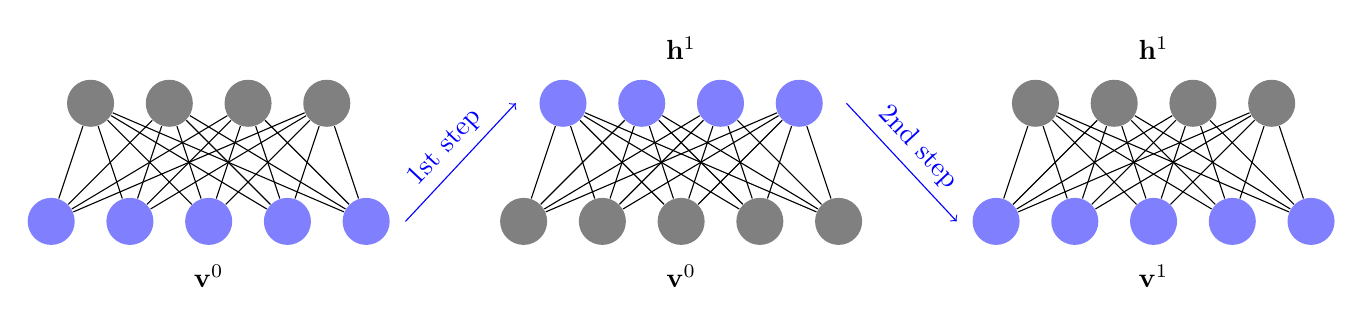
\begin{tikzpicture}[darkstyle/.style={circle,fill=black!50,minimum size=20}]
    \tikzstyle{every pin edge}=[<-,shorten <=1pt]
    \tikzstyle{neuron}=[circle,fill=black!25,minimum size=17pt,inner sep=0pt]
    \tikzstyle{input neuron}=[neuron, fill=blue!50];
    \tikzstyle{hidden neuron}=[neuron, fill=black!50];
     \tikzstyle{shidden neuron}=[neuron, fill=blue!50];
          \tikzstyle{thidden neuron}=[neuron, fill=black!50];
    \tikzstyle{annot} = [text width=4em, text centered]

    % Draw the input layer nodes
    \foreach \name / \y in {1,...,5}
    % This is the same as writing \foreach \name / \y in {1/1,2/2,3/3,4/4}       
     \node[input neuron] (I-\name) at (-\y, 0) {};

    % Draw the hidden layer nodes
\foreach \name / \y in {1,...,4}
	\node[hidden neuron] (H-\name) at (-\y -.5, 1.5) {};

    \foreach \source in {1,...,5}
        \foreach \dest in {1,...,4}
            \path (I-\source) edge (H-\dest);
            
            
    % Draw the input layer nodes
    \foreach \name / \y in {1,...,5}
    % This is the same as writing \foreach \name / \y in {1/1,2/2,3/3,4/4}       
     \node[hidden neuron] (II-\name) at (-\y +6, 0) {};

    % Draw the hidden layer nodes
\foreach \name / \y in {1,...,4}
	\node[input neuron] (HH-\name) at (-\y -.5 +6, 1.5) {};

    \foreach \source in {1,...,5}
        \foreach \dest in {1,...,4}
            \path (II-\source) edge (HH-\dest);
            
% Draw the input layer nodes
    \foreach \name / \y in {1,...,5}
    % This is the same as writing \foreach \name / \y in {1/1,2/2,3/3,4/4}       
     \node[input neuron] (III-\name) at (-\y +12, 0) {};

    % Draw the hidden layer nodes
\foreach \name / \y in {1,...,4}
	\node[hidden neuron] (HHH-\name) at (-\y -.5 +12, 1.5) {};

    \foreach \source in {1,...,5}
        \foreach \dest in {1,...,4}
            \path (III-\source) edge (HHH-\dest);
            
            \draw[->, blue] (-.5,0) -- node[above,sloped] {1st step} (.9,1.5);
                \draw[->, blue] (-.9 + 6,1.5)-- node[above,sloped] {2nd step} (.5 + 6,0);
             
            \draw    (-3,-.7) node {$\mathbf{v}^{0}$};
          %  \draw    (-3,2.2) node {$\mathbf{h}^{0}$};
            \draw    (-3 + 6,-.7) node {$\mathbf{v}^{0}$};
            \draw    (-3 +6,2.2) node {$\mathbf{h}^{1}$};
            \draw    (-3+ 12,-.7) node {$\mathbf{v}^{1}$};
            \draw    (-3 +12,2.2) node {$\mathbf{h}^{1}$};
\end{tikzpicture}
\end{center}
  \caption[1]{The first step of the Gibbs sampler for the RBM for a particular data point $\mathbf{v}^0 \in \mathcal{D}$.}
  \label{fig:gibbsSampling}
\end{figure}

The approximation to the gradient by the single data point $\mathbf{v}^0$ in the case of CD-$k$ takes the form:
\begin{align}
\begin{split}
- \sum_\mathbf{h} p(\mathbf{h} | \mathbf{v}^0) \frac{\partial E(\mathbf{v}^0, \mathbf{h})}{\partial \mathbf{\theta}} +  \sum_{\mathbf{h}} p(\mathbf{h} | \mathbf{v}^k) \frac{\partial E(\mathbf{v}^k,\mathbf{h})}{\partial \mathbf{\theta}} 
\label{eq:gradientCD}
\end{split}
\end{align}
It should be noted here that as we run the Gibbs chain only a few ($k$) steps, the samples $\{\mathbf{v}^k, \mathbf{h}^k\}$ don't come from the stationary distribution and the approximation \ref{eq:gradientCD} is biased as it doesn't maximize the likelihood of the data but the difference of two KL-divergences \cite{hinton2002training}, \cite{fischer2012introduction}:
$$KL(Q | P) - KL (P_k| P)$$
where $Q$ is the empirical distribution and $P_k$ is the distribution after $k$ step of the Gibbs chain and this explains the name of the algorithm.
\subsection{Persistent contrastive divergence}  
It was observed that the contrastive divergence procedure still requires many steps to be run in order to learn a good generative model. The rate of learning might be significantly improved when we don't reinitialize the Markov chains with a new training batch in order to obtain a sample $\{\mathbf{v}_i^k\}_{i=1}^N$ where $N$ is the size of the batch but rather keep "persistent" chains (PCD) \cite{tieleman2008training}. Thus, the starting state for the Gibbs chain is equal to the last step from the previous update. The assumption made here is that between parameter updates, the model changes only slightly in terms of parameters' values\cite{neal1992connectionist}. Thus, the initialization from the last state of the Gibbs chain taken from the previous model should be closer to the model distribution. The empirical results suggest to keep one persistent chain per one training data point in a batch.

\section{Learning using extended mean field approximation}
The stochastic procedure described in the previous section can be exchanged with the fully deterministic approach as the log-likelihood in the case of the EMF approximation has the form:
\begin{align}
\begin{split}
\mathcal{L} = \ln P(\mathbf{v}) = F^c(\mathbf{v}) - F^{EMF}.
\end{split}
\label{eq:emfLL}
\end{align}
As the first term from \ref{eq:loglikelihood} can be computed explicitly, it is independent from the approach taken during training and we only have to derive the updates using the EMF approximation of the free energy.

Let's now fix visible and hidden magnetizations $\{ \mathbf{m}^v, \mathbf{m}^h \}$. The gradient of the log-likelihood w.r.t a coupling parameter $W_{ij}$ up to the third-order term is:
\begin{align*}
\begin{split}
\frac{\partial F^{EMF}}{\partial W_{ij}} = & -m_i^v m_j^h - W_{ij}^t(m_i^v - (m_i^v)^2)(m_j^h - (m_j^h)^2) \\
 & - 2W_{ij}^2 (m_i^v - (m_i^v)^2)(\frac{1}{2} - m_i^v)(m_j^h - (m_j^h)^2)(\frac{1}{2} - m_j^h),
\end{split}
\end{align*}
while the updates for the bias terms are just negative of the fixed-point magnetizations:
\begin{align}
\begin{split}\frac{\partial F^{EMF}}{\partial a_i} &= -m_i^v, \\
\frac{\partial F^{EMF}}{\partial b_j} & = -m_j^h.
\end{split}
\end{align}
Thus, the training procedure using a deterministic approach goes as follows: given a data point $\mathbf{v}$ we obtain expected values of the hidden units $\mathbf{h} = \text{sigm} ( W\mathbf{v} + \mathbf{b})$ which are starting points for magnetizations, i.e. $\mathbf{m}^v_0 = \mathbf{v}$ and $\mathbf{m}^{h}_0 = \mathbf{h}$. Then, we perform an iterative algorithm (which can have the form as presented in the previous chapter) until convergence to obtain magnetizations $\{ \mathbf{m}^v,\mathbf{m}^h\}$ that satisfy self-consistency relations. Those magnetizations can then be used to obtain gradient w.r.t the parameters of the model and to compute the approximation of the free energy.
 
\section{Approximating the log-likelihood}
The problems related with intractability of the partition function makes training such structure very difficult as we cannot observe directly progress of learning. Thus, we need to resort to some approximations. One of the most popular approaches to measure progress in training RBMs is due to Besag \cite{besag1972nearest} -- consider the following approximation of $n$-dimensional distribution
\begin{equation}
P(\mathbf{x}; \theta) = \prod_i p(x_i| x_1,...,x_{i-1};\theta) \approx \prod_i p(x_i | x_1, ..., x_{i-1}, x_{i+1},..., x_n;\theta) = \prod_i p(x_i| x_{-i} ;\theta) \coloneqq PL (\mathbf{x};\theta) 
\end{equation}
where the first equation comes from the chain rule and $x_{-i}$ denotes the set of all variables except variable $x_i$. We assume here that marginals given all other are independent of each other. The likelihood has then the form:
\begin{equation}
\ln PL(\mathbf{x}; \theta) = \sum_i \ln P(x_i | x_{i-1} ;\theta).
\end{equation}
If the analysed phenomena has many dimensions this approximation is still computationally expensive. Thus, another step is to choose only one marginal as a proxy, i.e.
\begin{equation}
\ln PL(\mathbf{x}; \theta) = n \ln P(x_i | \mathbf{x}_{-i} ; \theta),
\end{equation}
where $i$ is randomly chosen from $\{1,2, ..., n\}$. It can be shown that this pseudo-likelihood is maximized by the true parameters of the model. In the case of the RBM, this estimator takes especially efficient form:
\begin{align}
\begin{split}
\ln PL(\mathbf{x}; \theta) \approx n \log \left( \frac{\exp\{- F^c(\mathbf{x})\}}{\exp\{-F^c(\mathbf{\hat{x}})\} + \exp\{- F^c(\mathbf{x})\}} \right) = n \ln \left( \text{sigm}(F^c(\mathbf{\hat{x}}) - F^c(\mathbf{x}) \right)
\label{eq:pseudoLL}
\end{split}
\end{align}
where $\mathbf{\hat{x}}$ represents the vector $\mathbf{x}$ with $i$-th variable flipped, i.e. $1-x_i$.

\section{Real scale model -- MNIST data set}
The data set that will be used for the comparison and the evaluation of EMF and CD training algorithms is the MNIST set \cite{lecun1998} which is a well-known benchmark image classification dataset that consists of $60000$ training and $10000$ testing images of digit numbers. They are represented
on $28$-by-$28$ grey-scale grid of pixels. Thus, the first visible layers in all analysed models consists of $784$ visible units. Following \cite{gabrie2015training}, \cite{salakhutdinov2008learning} all images were rescaled to $ \lbrace 0, 1 \rbrace $ and binarized by setting all non-zero pixels to $1$ in all experiments.
The data set was divided into $600$ mini-batches which results in $100$ training points per batch.

\subsection{Comparison of both approaches}
In order to test the efficiency of the EMF learning algorithm, I used three expansions of $\ref{eq:varFreeEnergy}$ -- up to the first-order (MF), second-order (TAP2) and third order (TAP3) term. Moreover, I varied the number of iterations of self-consistency relations ($3$ and $10$) using asynchronous updates of the form \ref{eq:asynch} to mimic the idea from the contrastive divergence approach. As a benchmark, two models were trained following the stochastic training (CD$1$, CD$10$).

Furthermore, all models described above were trained using persistent approach (PMF, PTAP2, PTAP3, PCD). In the case of the EMF approximation, the magnetizations of a batch  from the previous update are the starting points in the next update \cite{gabrie2015training}. Similarly to PCD, this idea is based on the fact that between updates the model changes only slightly and it should improve the convergence to the new fixed point magnetizations.

All models were trained $10$ times using the same set-up of free parameters with $500$ units. The purpose of this experiment is to compare different RBM trainings thus following \cite{gabrie2015training} I didn't use the adaptive learning rate which was set to $0.005$, learning was performed using mini-batch updates with $100$ training points per batch. The couplings matrix was randomly initialised using normal distribution with zero mean and variance set to $0.01$. This allows to compare the procedures in the their "raw" forms. 

However, the EMF approximation was performed around the infinite temperature were the spins are independent. Thus, in general couplings should have small values -- this can be enforced using regularization which at the same times allows for a better generalization. From probabilistic perspective this can be seen as adding a weighted prior over the parameters (maximum a posteriori training). The criterion that will be maximized has now the form:
\begin{align}
\begin{split}
E(\theta, \mathcal{D}) = \ln \mathcal{L}(\mathbf{\theta}| \mathcal{D}) - \lambda R(\theta)
\end{split}
\end{align}
where $R(\cdot)$ is the regularizer and $\lambda \in \mathbb{R}_+$ is a hyper-parameter which controls the effective power of the regularization.
In all experiments Laplacian prior $R(\theta) = \| \theta \|_1$ ($L1$ regularization) was used with $\lambda$ set to $0.01$. 

Figure \ref{fig:validLL} presents the pseudo log-likelihood \ref{eq:pseudoLL} (left) and EMF log-likelihood \ref{eq:emfLL} for the non-persistent training procedure. Firstly, by the visual inspection both approximation yield very similar results for each analysed model. However, the EMF estimates are much less noisy at a lower computational cost.

\begin{figure}[!htb]
\minipage{0.50\linewidth}%
%  \includegraphics[width=\linewidth]{../../../Code/DRBM/scripts/validLL}
\endminipage 
\minipage{0.50\linewidth}  
 %\includegraphics[width=\linewidth]{../../../Code/DRBM/scripts/validEMF}
\endminipage\hfill
  \caption[1]{Per-sample pseudo log-likelihood (left) and EMF log-likelihood (right) on the validation set of the MNIST data set divided by number of all units in the model ($1284$) across first training $50$ epochs for RBMs models trained stochastically and deterministically. Error bars shows the standard deviations of $10$ trained models using a particular version of training.}
   \label{fig:validLL}
\end{figure}
Secondly, results for the MF-10\footnote{The results for MF-3 weren't included as it was very similar to the MF-10} confirms the findings from the literature -- the naive mean field approach is not able to learn an effective model. Moreover, the results for the CD, TAP2 and TAP3 are very similar. There are not significant differences between models with $3$ or $10$ iterations of self-consistency relations which shows that the deterministic approach is not computationally expensive. 

As it was expected, the best results in terms of the EMF log-likelihood are achieved by EMF methods. However, the results for the CD models suggest that the EMF log-likelihood may be used as a reliable indicator of progress during training as those models weren't constructed to optimize over this objective \cite{gabrie2015training}.

Figure \ref{fig:PvalidLL} presents the results for persistent versions of models analysed above. There are not significant differences comparing to However, as it was expected the samples from the models trained using persistent chains are of much higher quality.
\begin{figure}[!htb]
\minipage{0.50\linewidth}
 \includegraphics[width=\linewidth]{../../../Code/DRBM/scripts/PvalidLL}
\endminipage 
\minipage{0.50\linewidth}  
 \includegraphics[width=\linewidth]{../../../Code/DRBM/scripts/PvalidEMF}
\endminipage\hfill
  \caption[1]{Per-sample pseudo log-likelihood (left) and EMF log-likelihood (right) for the same models trained using persistent Gibbs chains. Results of the naive method weren't included.}
   \label{fig:PvalidLL}
\end{figure}

Finally, in persistent and non-persistent versions of models the addition of the third order term from the EMF expansion \ref{eq:EMFexpansion} doesn't provide improvement over the TAP model. This might be partially explained by the fact that estimated weights are in general smaller than $1$ (in absolute value) which are then used at the order of $3$ in self-consistency equations and hence don't affect significantly estimations.

\subsection{Generated samples from the models}
The restricted Boltzmann machine can also be seen as a generative model that can creates new samples that will resemble the observed data provided that it approximates well the unknown distribution that generated the original, observed samples. Three models were trained with $500$ hidden units using persistent chains -- with the contrastive divergence algorithm, and two models using naive and extended mean field approach respectively. Figure \ref{fig:particles} shows samples generated from those models where between samples $1000$ chain steps were performed.
\begin{figure}[!htb]
\minipage{0.46\linewidth}%
 \includegraphics[width=\linewidth]{../../../Code/DRBM/backup/org/particles}
\endminipage 
\hfill
\minipage{0.46\linewidth}  
 \includegraphics[width=\linewidth]{../../../Code/DRBM/backup/mf/particles}
\endminipage
\vspace{2em}
  \minipage{0.46\linewidth}%
 \includegraphics[width=\linewidth]{../../../Code/DRBM/backup/pcd/particles}
\endminipage 
\hfill
\minipage{0.46\linewidth}  
 \includegraphics[width=\linewidth]{../../../Code/DRBM/backup/tap2/particlestap2}
\endminipage
  \caption[1]{Comparison of samples generated by $500$ hidden unit RBM trained using naive mean field approach (top right), extended mean field approximation up to the second-term order (bottom right) and with contrastive divergence (bottom left) to the original digits from the MNIST data (top left). All models were trained using persistent chains.}
  \label{fig:particles}
\end{figure}
The samples produced by the naive mean field methos provides the samples of the poorest quality that are often non-identifiable as one of $10$ digits. As we can see, the addition of the second-order term greatly improves also the generetive qualitative of the learned model. It might be argued that samples produced by the PCD and EMF models are of similar quality.
